%!TEX TS-program = xelatex

%%%%%%%%%%%%%%%%%%%%%%%%%%%%%%%%%%%%%%%%%%%%%%%%
% CV template
% Originally created by Adrien Friggeri
% Improved by Carmine Benedetto
%%%%%%%%%%%%%%%%%%%%%%%%%%%%%%%%%%%%%%%%%%%%%%%%

\documentclass[]{cv-class}
\usepackage{afterpage}
\usepackage{hyperref}
\usepackage{color}
\usepackage{xcolor}
\hypersetup{
    colorlinks=true,
    linkcolor=blue
}
\addbibresource{bibliography.bib}
\RequirePackage{xcolor}

\usepackage[utf8]{inputenc}
\usepackage[english]{babel}
 
\usepackage[usenames, dvipsnames]{color}

\begin{document}

% In the aside, each new line forces a line break
\begin{aside}
\color{blue}
  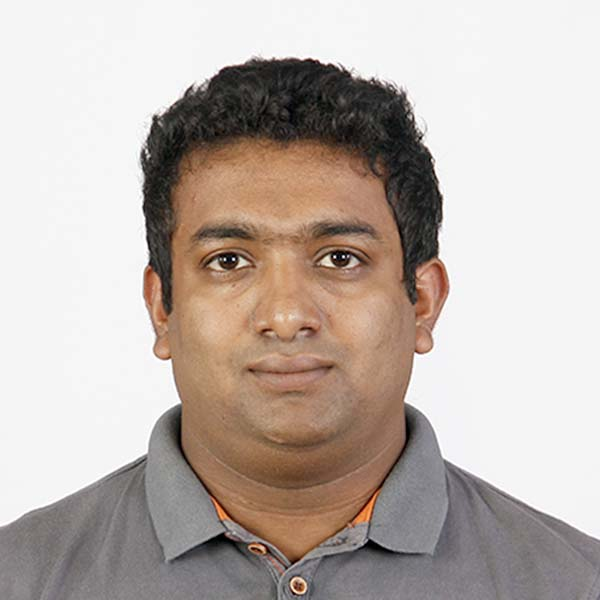
\includegraphics[scale=0.9]{img/photo.jpg}
    ~
  \header{Janitha}{Madushan}
      {Software Engineer}
   ~
  \section{Address}
    {\whitebodyfont No:04, "Sunhill,"\\
    Vajirapura,\\
    Nuwara-Eliya\\
    Sri-Lanka}
    ~
  \section{Phone}
    {\whitebodyfont +94 71 57 81 553\\
    +94 75 97 46 502}
    ~
  \section{Mail}
    \underline{\href{mailto:janithasen@gmail.com}{{\whitebodyfont janithasen@gmail.com}}}
    ~
  \section{Web}
  	\vspace{0.10cm}
    \underline{\href{https://www.linkedin.com/in/janithamadushan}{{\whitebodyfont linkedin}}}
    \\
	\vspace{0.10cm}
    \underline{\href{https://stackoverflow.com/story/jmadushan}{{\whitebodyfont stackoverflow}}}
	\\	
	\vspace{0.10cm}
    \underline{\href{https://github.com/janitham}{{\whitebodyfont github}}}
    ~
  \section{Langauges}
  	{\whitebodyfont Sinhaleese (Native)\\
    Engilsh}
    ~
  \section{Civil status}
    {\whitebodyfont Married}
  	~  
  \section{OS Preference}
    \asidelist{{\whitebodyfont Windows}}
    {\includegraphics[scale=0.30]{img/star.png}
    \includegraphics[scale=0.30]{img/star.png}
    \includegraphics[scale=0.30]{img/star.png}
    \includegraphics[scale=0.30]{img/star.png}
    \includegraphics[scale=0.30]{img/star.png}}
    \asidelist{\whitebodyfont{Linux}}
    {\includegraphics[scale=0.30]{img/star.png}
    \includegraphics[scale=0.30]{img/star.png}
    \includegraphics[scale=0.30]{img/star.png}
    \includegraphics[scale=0.30]{img/star_empty.png}
    \includegraphics[scale=0.30]{img/star_empty.png}}
    ~
  \section{Programming}
    \asidelist{{\whitebodyfont Java}}
    {\includegraphics[scale=0.30]{img/star.png}
    \includegraphics[scale=0.30]{img/star.png}
    \includegraphics[scale=0.30]{img/star.png}
    \includegraphics[scale=0.30]{img/star.png}
    \includegraphics[scale=0.30]{img/star_empty.png}}
    \asidelist{\whitebodyfont{C}}
    {\includegraphics[scale=0.30]{img/star.png}
    \includegraphics[scale=0.30]{img/star.png}
    \includegraphics[scale=0.30]{img/star.png}
    \includegraphics[scale=0.30]{img/star.png}
    \includegraphics[scale=0.30]{img/star_empty.png}}
    \asidelist{\whitebodyfont{Pyhon}}
    {\includegraphics[scale=0.30]{img/star.png}
    \includegraphics[scale=0.30]{img/star.png}
    \includegraphics[scale=0.30]{img/star.png}
    \includegraphics[scale=0.30]{img/star_empty.png}
    \includegraphics[scale=0.30]{img/star_empty.png}}
    \asidelist{\whitebodyfont{.NET}}
    {\includegraphics[scale=0.30]{img/star.png}
    \includegraphics[scale=0.30]{img/star.png}
    \includegraphics[scale=0.30]{img/star.png}
    \includegraphics[scale=0.30]{img/star_empty.png}
    \includegraphics[scale=0.30]{img/star_empty.png}}
    \asidelist{\whitebodyfont{PHP}}
    {\includegraphics[scale=0.30]{img/star.png}
    \includegraphics[scale=0.30]{img/star.png}
    \includegraphics[scale=0.30]{img/star.png}
    \includegraphics[scale=0.30]{img/star_empty.png}
    \includegraphics[scale=0.30]{img/star_empty.png}}
    ~
\end{aside}

\section{Experience}
\begin{entrylist}
  \entry
    {Nov. 15 - Now}
    {Software Developer}
    {Cambio Software Engineering}
    {I am working in automation team in configuration management team as a software developer. My responsibility 
    is to automate manual tasks in continuous delivery, continuous integration and management tools. On that tasks
    I developed various tools using various technologies. Mainly I developed tools using maven-plugins(MOJO), JAVA 
    and various devops technologies. Recently I am working in "Git Migration" sub project in "Tiger Infrastructure Project"\\}
  \entry
    {Oct. 15 - March. 16}
    {Internship}
    {IFS RD}
    {I worked with "Technology" team and two distinct internal projects during my internship. I developed one internal
	application and a research project. In that period I exposed to ASP.NET, ORACLE 11G/12C, PLSQL, ANDROID and JAVA.}
\end{entrylist}

\section{Education}
\begin{entrylist}
  \entry
    {Aug. 11 - June 15}
    {Bsc(Hons.) Computer Engineering}
    {Faculty of Engineering, University of Peradeniya}
    {I followed computer engineering at Faculty of engineering of University of peradeniya. There I specified in computer 		   	engineering also specified in software engineering}
\end{entrylist}



\section{Projects}
\begin{entrylist}
  \entry
    {Oct. 16 - Now}
    {Package Automation tool\#}
    {Stacker}
    {Package automation tool}
  \entry
    {Aug. 15 - Oct. 15}
    {Packaging data management tool}
    {Snooper}
    {Snooper}
  \entry
    {June 15}
    {Device dependent CAPTHCHA System}
    {Final Year Project}
    {CAPTCHA system that provides suitable CAPTCHAs for suitable devices
	by  detecting  the  device,  then  provides  the  CAPTCHAs  as  their 
	functionalities and usability.}
  \entry
    {June 15}
    {IFS Rest Data service}
    {Internship Project}
    {Research on exposing database hosted server  APIs  as  RESTful  services. 
	Demonstrated  using  MS  excel  office  application}
  \entry
    {June 15}
    {IFS Day-Care Application}
    {Final Year Project}
    {Web  based  application  used  by  IFS  employees  to  reserve  the  day-care 
	facility at IFS. (Used ASP.NET, PLSQL, Oracle 11g database, Android, 
	Java)}
  
\end{entrylist}

\newpage

\begin{aside}
\end{aside}

\begin{entrylist}
  \entry
    {Oct. 16 - Now}
    {Package Automation tool\#}
    {Stacker}
    {Package automation tool}
  \entry
    {Aug. 15 - Oct. 15}
    {Packaging data management tool}
    {Snooper}
    {Snooper}
  \entry
    {June 15}
    {Device dependent CAPTHCHA System}
    {Final Year Project}
    {CAPTCHA system that provides suitable CAPTCHAs for suitable devices
	by  detecting  the  device,  then  provides  the  CAPTCHAs  as  their 
	functionalities and usability.}
  \entry
    {June 15}
    {IFS Rest Data service}
    {Internship Project}
    {Research on exposing database hosted server  APIs  as  RESTful  services. 
	Demonstrated  using  MS  excel  office  application}
  \entry
    {June 15}
    {IFS Day-Care Application}
    {Final Year Project}
    {Web  based  application  used  by  IFS  employees  to  reserve  the  day-care 
	facility at IFS. (Used ASP.NET, PLSQL, Oracle 11g database, Android, 
	Java)}
\end{entrylist}

\section{References}
\begin{entrylist}
  \entry
    {}
    {}
    {}
    {Upon Request}
\end{entrylist}


\vspace{1.5cm}
\begin{flushright}
\emph{Janitha Madushan}
\end{flushright}
\begin{flushright}
\emph{\today}
\end{flushright}

\end{document}
